In this section comparisons between the models described in this report are done. In particular as said in \ref{chapter:code-setup} the results of the algorithms are analyzed using the performance profile tool provided. Several runs were carried out to fully test the models so that a more accurate conclusion is collected. In particular, the best algorithm is the one that finds the optimal solution in the shortest time for the most times. While analyzing the metaheuristics approaches it is impossible to compare them in a time scale, so instead of the time the comparison is done between the cost of the solution obtained by each model.

Since the TSP is an NP-hard problem finding a winner is not always so easy. Sometimes different methods can lead to very similar results, so while analyzing it is going to be taken up into consideration several factors such as consistency.

To discuss the outcome of the tests is plotted and so it is needed some explanation on how to understand them. While the x-axis portrays the time (or cost) ratio which will show what algorithm performs better, the y-axis shows the fraction of instances that the algorithm ends up winning. In general, the best method is the one that can remain on the left side of the chart consistently.

As explained in section \ref{sec:solution-data-management} the TSPLIB is used only to carry out if the implemented algorithms can reach the optimal value. To run these tests a series of randomly generated instances are used.

\section{Compact models}
\label{sec:results-compact}
In this section the compact models presented in chapter \ref{chapter:compact-models} focusing in particular of MTZ and its variants and GG models. To test them a set of 20 instance of 50 nodes were generated and runned with a global timelimit of 30 minutes. The results are visible in figure \ref{fig:result-compact}.

\begin{figure}[h]
	\centering
	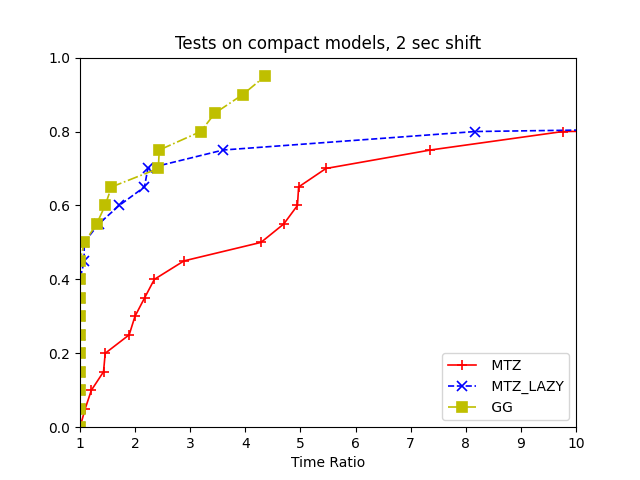
\includegraphics[width=0.6\textwidth]{images/final_mtz_mtzlazy_gg.png}
	\caption{The comparison chart of the compact models.}
	\label{fig:result-compact}
\end{figure}

From this image we can state that the MTZ basic model is far from being the best one of this section. In fact the best models are GG and MTZ\_LAZY wich on many instaces perform in a comparable way. But it is possible to see that while MTZ\_LAZY in some cases as reached the timelimit, the GG model deliver a consistent solution of the instance.
